% Options for packages loaded elsewhere
\PassOptionsToPackage{unicode}{hyperref}
\PassOptionsToPackage{hyphens}{url}
\PassOptionsToPackage{dvipsnames,svgnames,x11names}{xcolor}
\documentclass[
  10pt,
  fontset=fandol]{ctexart}
\usepackage{xcolor}
\usepackage[margin=16mm]{geometry}
\usepackage{amsmath,amssymb}
\setcounter{secnumdepth}{-\maxdimen} % remove section numbering
\usepackage{iftex}
\ifPDFTeX
  \usepackage[T1]{fontenc}
  \usepackage[utf8]{inputenc}
  \usepackage{textcomp} % provide euro and other symbols
\else % if luatex or xetex
  \usepackage{unicode-math} % this also loads fontspec
  \defaultfontfeatures{Scale=MatchLowercase}
  \defaultfontfeatures[\rmfamily]{Ligatures=TeX,Scale=1}
\fi
\usepackage{lmodern}
\ifPDFTeX\else
  % xetex/luatex font selection
\fi
% Use upquote if available, for straight quotes in verbatim environments
\IfFileExists{upquote.sty}{\usepackage{upquote}}{}
\IfFileExists{microtype.sty}{% use microtype if available
  \usepackage[]{microtype}
  \UseMicrotypeSet[protrusion]{basicmath} % disable protrusion for tt fonts
}{}
\makeatletter
\@ifundefined{KOMAClassName}{% if non-KOMA class
  \IfFileExists{parskip.sty}{%
    \usepackage{parskip}
  }{% else
    \setlength{\parindent}{0pt}
    \setlength{\parskip}{6pt plus 2pt minus 1pt}}
}{% if KOMA class
  \KOMAoptions{parskip=half}}
\makeatother
\usepackage{graphicx}
\makeatletter
\newsavebox\pandoc@box
\newcommand*\pandocbounded[1]{% scales image to fit in text height/width
  \sbox\pandoc@box{#1}%
  \Gscale@div\@tempa{\textheight}{\dimexpr\ht\pandoc@box+\dp\pandoc@box\relax}%
  \Gscale@div\@tempb{\linewidth}{\wd\pandoc@box}%
  \ifdim\@tempb\p@<\@tempa\p@\let\@tempa\@tempb\fi% select the smaller of both
  \ifdim\@tempa\p@<\p@\scalebox{\@tempa}{\usebox\pandoc@box}%
  \else\usebox{\pandoc@box}%
  \fi%
}
% Set default figure placement to htbp
\def\fps@figure{htbp}
\makeatother
\setlength{\emergencystretch}{3em} % prevent overfull lines
\providecommand{\tightlist}{%
  \setlength{\itemsep}{0pt}\setlength{\parskip}{0pt}}
\usepackage{amsmath,amssymb,mathtools,needspace}
\xeCJKDeclareCharClass{CJK}{"2032,"0400->"04FF,"2160->"216B,"2460->"2473,"25A0,"25C7,"25CB,"25CF}
\IfFontExistsTF{Arial Unicode MS}{\xeCJKsetup{AutoFallBack=true}\setCJKfallbackfamilyfont{\CJKrmdefault}{Arial Unicode MS}}{}
\setcounter{secnumdepth}{0}
\setlength{\emergencystretch}{2em}
\allowdisplaybreaks
\usepackage{bookmark}
\IfFileExists{xurl.sty}{\usepackage{xurl}}{} % add URL line breaks if available
\urlstyle{same}
\hypersetup{
  pdftitle={Milne 格式},
  colorlinks=true,
  linkcolor={Maroon},
  filecolor={Maroon},
  citecolor={Blue},
  urlcolor={Blue},
  pdfcreator={LaTeX via pandoc}}

\title{Milne 格式}
\author{}
\date{}

\begin{document}
\maketitle

\subsubsection{5.5.6 Milne 格式}\label{milne-ux683cux5f0f}

与格式（5.5.19）不同的另一类格式是用 \(y_{n-3}\) 而不用 \(y'_{n-3}\)，其形式为

\[
y_{n+1}=\alpha_0y_n+\alpha_1y_{n-1}+\alpha_2y_{n-2}+\alpha_3y_{n-3}+h(\beta_0y'_n+\beta_1y'_{n-1}+\beta_2y'_{n-2}).
\tag{5.5.23}
\]

类似于前面的讨论，运用 Taylor 展开方法不难导出形如式（5.5.23）的一类四阶方法。这类方法中包含有著名的 Milne 格式

\[
y_{n+1}=y_{n-3}+\frac{4h}{3}(2y'_n-y'_{n-1}+2y'_{n-2}),
\tag{5.5.24}
\]

其局部截断误差为

\[
y(x_{n+1})-y_{n+1}\approx\frac{14}{45}h^5y_n^{(5)}.
\tag{5.5.25}
\]

Milne 格式也可以通过数值积分的途径推导出来。事实上，从积分恒等式

\[
y(x_{n+1})=y(x_{n-3})+\int_{x_{n-3}}^{x_{n+1}}y'(x)\,\mathrm dx
\tag{5.5.26}
\]

着手，用数据点 \((x_n,\allowbreak y'_n),\allowbreak (x_{n-1},\allowbreak y'_{n-1}),\allowbreak (x_{n-2},\allowbreak y'_{n-2})\) 插出二次式 \(P_2(x)\)，然后用 \(P_2(x)\) 替代 \(y'(x)\) 计算式（5.5.26）中的积分项，即可得到上述格式（5.5.24）。

再在形如式（5.5.21）的四阶隐式方法中适当挑选一个与 Milne 格式相匹配。在式（5.5.22）中令 \(\alpha_1=1,\alpha_2=0\)，可定出下列四阶格式：

\begin{quote}
校注（agent 补充，ch05b-E005）：式（5.5.21）右端开头在原图中印作 \(\alpha_0y_{n+1}\alpha_1y_{n-1}\)（``\(+1\)''下沉至下标位置，且两项之间无正常加号），上式按可见字形保留。由本页``舍弃 \(y'_{n-3}\) 而代之以 \(y'_{n+1}\)''及式（5.5.19）、（5.5.22），此处疑为排印错误，预期应是 \(\alpha_0y_n+\alpha_1y_{n-1}\)。局部原图如下，仅用于保存这一排印疑误的可审计证据。
\end{quote}

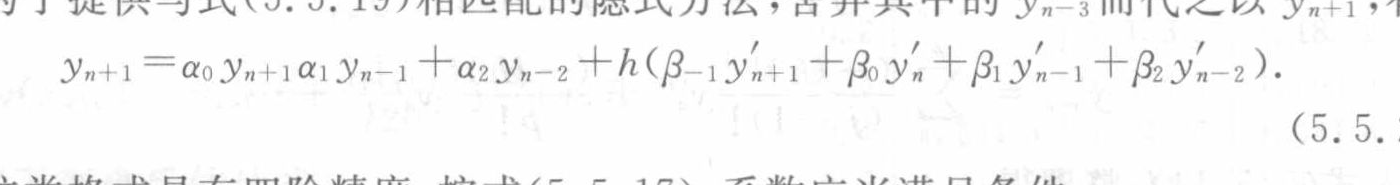
\includegraphics[width=0.85\linewidth,height=\textheight,keepaspectratio,alt={式（5.5.21）原图局部：右端开头的下标与加号排印异常}]{../assets/ch05b/pdf-143-eq521.png}

\href{../../source-images/pdf-144.jpeg}{原页}

\[
y_{n+1}=y_{n-1}+\frac h3(y'_{n+1}+4y'_n+y'_{n-1}).
\tag{5.5.27}
\]

上述格式通常称为 Simpson 格式，用数值积分的 Simpson 方法处理积分恒等式

\[
y(x_{n+1})=y(x_{n-1})+\int_{x_{n-1}}^{x_{n+1}}y'(x)\,\mathrm dx
\]

即可导出这一格式。

用 Simpson 格式（5.5.27）与 Milne 格式（5.5.24）匹配，构成下列预测-校正系统：

预测

\[
\bar y_{n+1}=y_{n-3}+\frac{4h}{3}(2y'_n-y'_{n-1}+2y'_{n-2}),\qquad
\bar y'_{n+1}=f(x_{n+1},\bar y_{n+1});
\]

校正

\[
y_{n+1}=y_{n-1}+\frac h3(\bar y'_{n+1}+4y'_n+y'_{n-1}),\qquad
y'_{n+1}=f(x_{n+1},y_{n+1}).
\]

\subsection{本节覆盖原页的校注记录}\label{ux672cux8282ux8986ux76d6ux539fux9875ux7684ux6821ux6ce8ux8bb0ux5f55}

下列记录按原页关联，含同页相邻小节的校注；计算时同时读取上文校注和完整原页。

\begin{itemize}
\tightlist
\item
  \texttt{ch05b-E005}：原书 PDF 页 143
\end{itemize}

\end{document}
